\documentclass[sigconf]{acmart}

\usepackage{hyperref}

%\usepackage{endfloat}
%\renewcommand{\efloatseparator}{\mbox{}} % no new page between figures

\usepackage{booktabs} % For formal tables

\settopmatter{printacmref=false} % Removes citation information below abstract
\renewcommand\footnotetextcopyrightpermission[1]{} % removes footnote with conference information in first column
\pagestyle{plain} % removes running headers


\begin{document}
\title{Big Data Analysis in Finance Sector}


\author{Dhanya Mathew}
\orcid{HID328}
\affiliation{%
  \institution{Indiana University}
  \streetaddress{711 N Park Ave}
  \city{Bloomington} 
  \state{Indiana} 
  \postcode{47408}
}
\email{dhmathew@iu.edu}

% The default list of authors is too long for headers}
\renewcommand{\shortauthors}{B. Trovato et al.}


\begin{abstract}

Big data as the name implies, refers to large and complex data which continues to grow enormously day by day. The broad proliferation of data and new and efficient technological support has transformed the way industries operate and compete. Industries like financial firms, in particular, have widely adopted big data analytics to obtain better investment decisions with consistent growth. In order to understand what drives profit in an organization or company, we should be able to predict the business trends, challenges, opportunities risks and what profit group (extremely unprofitable, average, extremely profitable etc.) a set of customers falls into based on their data at any given time. Financial firms like banks are storing these data for many decades and the recent technology boom that happened with big data technologies help the firms to uncover the secrets to understand consumer behavior, prevent major disasters and theft. We show the wide possibilities open for financial firms by analyzing big data to improve decision making, productivity, customer satisfaction etc which in turn beneficial for both organizations and customers.
\end{abstract}

\keywords{i523, HID328, big data, data-driven, data lakes, Hadoop, Random Forest}


\maketitle

\section{Introduction}

There are 3 fundamental elements to big data - Volume, Variety and Velocity. Velocity is the speed at which data must be stored and analyzed\cite{how-big-data-has-changed-finance}. Data sets grow rapidly because they are increasingly gathered by cheap and numerous information-sensing Internet of things devices such as mobile devices, aerial (remote sensing), software logs, cameras, microphones, radio-frequency identification (RFID) readers and wireless sensor networks\cite{wiki-bigdata}. According to 2015 big data info graphic contributed by Ben Walker of Voucher Cloud, around 2.5 quintillion Bytes of data is created every day which would fill 10 million Blu-ray discs. These discs when stacked on one another, would measure the height of 4 Eiffel Towers. Ben suggests that data generation by 2018 will be 50,000 GB per second\cite{how-much-data-is-created-daily}. 

According to Gartner Survey, 64 percent of organizations invested or planning to invest in big data technology in 2013(including but not limited to Hadoop, NoSQL, Spark, R and Storm)\cite{gartner-survey}. Recent survey research indicates that 71 percent of firms in the financial services
industry at a global level are exploring Big
Data and predictive analytics\cite{accenture-next-generation-financial}. This number continues to grow and sectors like government, business, technology, universities, health-care, finance, manufacturing etc make use of big data to obtain meaningful information using big data technologies\cite{wiki-bigdata}. We investigate in particular, how big data is helpful in financial firms in terms of predictive analysis and profitable growth. The finance sector also contributes to the daily data generation from products and marketing, banking, business, share market etc. Finance is a very sensitive field and any useful insight can make a positive impact on the overall turnover. Historic data analysis and real time data analysis are equally important in terms of finance sector. The key idea behind is how to retrieve the 'signal' of relevant information form the bulk of data. Let us explore the wide range of possibilities of big data analysis that finance sector can come up with including decision making, discovery of new business opportunities, enhanced productivity and efficiency, risk management, fraud detection, innovation possibilities, efficiency and growth and customer segmentation.

\subsection{Efficient Decision Making}

The era of big data helps financial firms to take quality business decisions related to expanding revenues, managing costs, hiring resources etc. based on effective data analysis which provide access to real-time insights.  Data-driven decision making is one of the key advantages of big data technologies. Data driven decision making approach includes data storage, data elaboration, data analysis and decision making\cite{accenture-next-generation-financial}.`

\begin{figure}[htb]
  \centering
  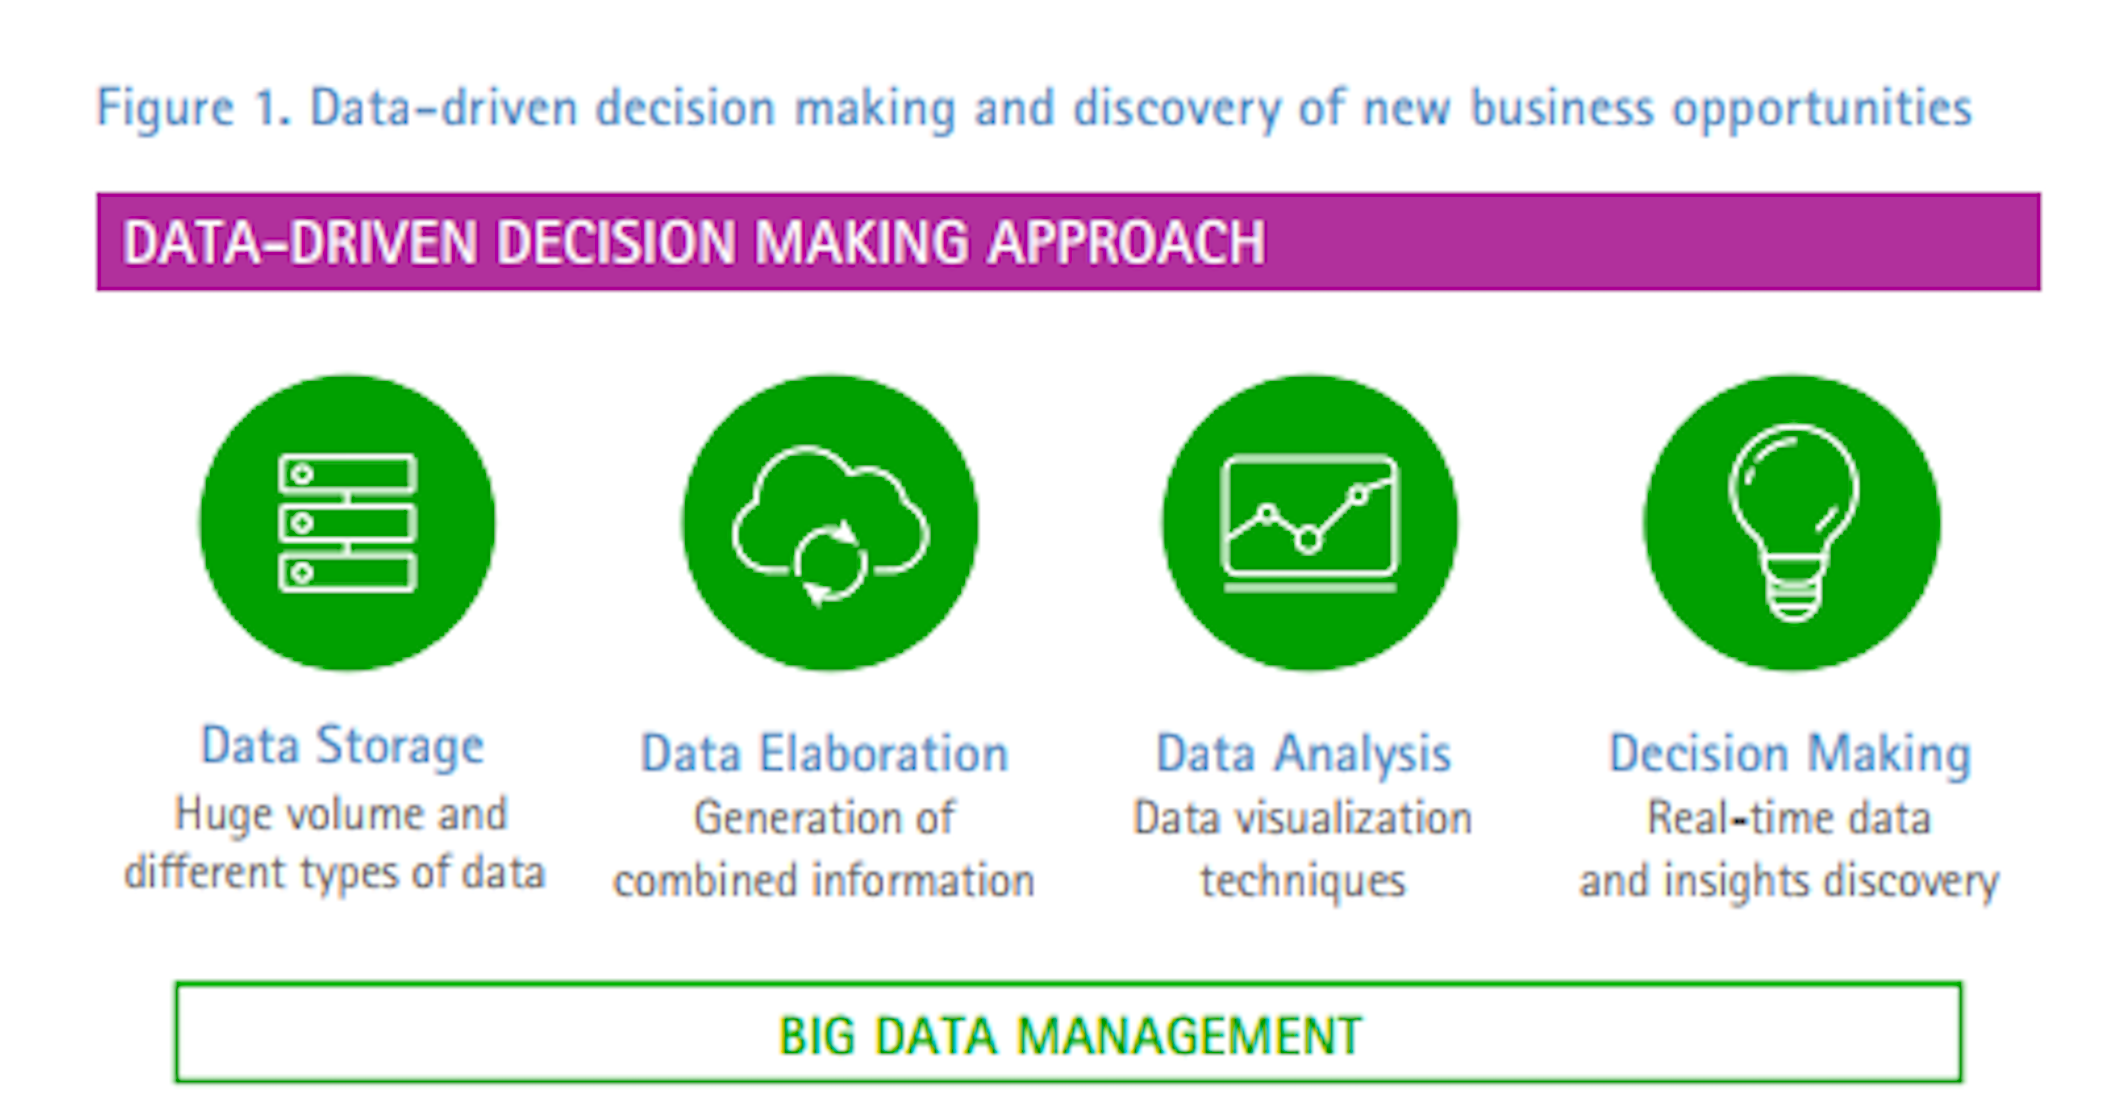
\includegraphics[width=1.0\columnwidth]{images/Figure1.png}
  \caption{Data-driven decision making approach 
  \cite{accenture-next-generation-financial}}
  \label{fig:Figure1} 
\end{figure}

Figure 1 \TODO{USE ref} shows data-driven decision making approach and discovery of new business opportunities.

\textit{Data Storage:} Even though big data does not define by the size alone, we need the right means to store the huge volume and variety of data. Big data is distributed - stored across many machines and managed with Hadoop File System and distributed DBs like HBase and Apache Cassandra\cite{big-data-storage}.

\textit{Data Elaboration:} Generate combined information by eliminating unwanted data using data cleansing methods like grouping, joining, filtering etc.(Spark, R, MapReduce, Storm). 

\textit{Data Analysis:} Big data analysis is the process of analyzing the data to derive the semantics of the available data to understand the hidden patterns, correlations, market trends, customer preferences which helps the organizations to take more informed decisions. Visualization tools include- Tableau, Google chart, D3, Fusion chart etc. are used to visualize the results of analysis.

\textit{Decision Making:} Data-driven decision making based on the analysis.
 
 There is a feedback analysis done for a bank as part of 2nd International Symposium on Big Data and Cloud Computing. Feedback processes are important for any organization to help and understand the potential areas of improvement and if done on a regular basis, they help to identify gaps in services rendered. This bank also started to collect feedback from their customers over a period of 3 years and 6 months; from those who visited bank branches as well as from those who used online services. Customers were asked to rate the bank anonymously on a scale of 1 to 5 on the following parameters: 
 
\begin{itemize}
   \item Is the customer happy with the quality of service?
   \item Is the customer happy with the speed of service?
   \item Are customer queries addressed effectively?
\end{itemize}

The analysis is performed using the pertaining subset of the total data collected, comprising of feedback from around 20,000 customers\cite{bigdata-banking}. 

\begin{figure*}[htb]
  \centering
  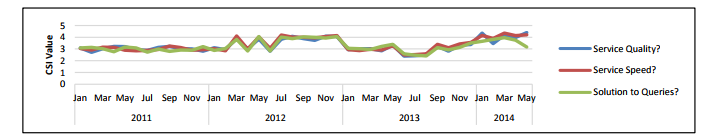
\includegraphics[width=1.0\textwidth]{images/Figure2.png}
  \caption{Overall Customer Feedback for provided parameters 
  \cite{bigdata-banking}}
  \label{fig:Figure2} 
\end{figure*}

As shown in Figure 2 \TODO{USE ref}, the customers rated bank services as average. Hence the concerned bank took some measures to correct the issue, and this resulted in ratings improvements.

\subsection{Increased Productivity and Growth}
Compared to traditional data warehouses, the big data concept of Data lakes to store raw data offers more flexibility in data access and analysis. Large volumes of data are stored, managed and analyzed in data lakes  by using automated and sophisticated analytical tools. 

Applications like, Machine learning algorithms, In-memory technologies, fast access DBs, big data queries and real-time analysis methods consume less time to come up with meaningful information and reports by accessing data lakes.

\textit{Data Lakes:} Data Lakes can be compared to the actual lakes where rivers or streams that bring water to it. In data lakes, this is called ingestion of data. We collect all the data that we require to analyze to reach our goal irrespective of the source. These 'streams' of data come in several formats: structured data (simply said, data from a traditional relational database or even spreadsheet: rows and columns), unstructured data (social, video, email, text etc.), data from all sorts of logs (weblogs, clickstream analysis etc.), XML, machine-to-machine, IoT and sensor data. Logs and XML are also called semi-structured data. There can be data filters in place based on the requirements\cite{data-lakes}.

\subsection{Fraud Detection}
One of the best ways to fight cybercrime is with early detection. Banks are prime targets for cybercriminals and fraudsters, and any kind of public breach creates a lot of embarrassment, bad publicity, and unwanted scrutiny. Clearly banks have a vested interest in any technology to identify and prevent a data breach or fraud\cite{the-top-5-trends-for-big-data-in-financial-services}.

Banks and financial services firms use analytics to differentiate fraudulent interactions from legitimate business transactions. By applying analytics and machine learning, they are able to define normal activity based on a customer's history and distinguish it from unusual behavior indicating fraud. The analysis systems suggest immediate actions, such as blocking irregular transactions, which stops fraud before it occurs and improves profitability\cite{5-big-data-use-cases-in-banking-and-financial-services}.

The security and fraud analysis done by 2nd International Symposium on Big Data and Cloud Computing, clearly shows that, based on historical transactions and consumption capacity of customers, coupled with the behavioral analysis can help us reveal a potential threat to the system, as well as uncover frauds that might have happened in the past\cite{bigdata-banking}. 

\begin{figure*}[htb]
  \centering
  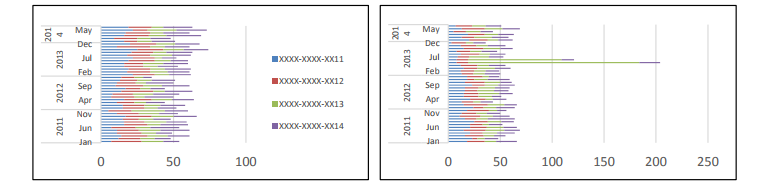
\includegraphics[width=1.0\textwidth]{images/Figure3.png}
  \caption{Net credit transactions count (left) and net debit transactions count (right) 
  \cite{bigdata-banking}}
  \label{fig:Figure3} 
\end{figure*}

As shown in Figure \ref{fig:Figure3} from the analysis, we can observe that net transactions count grows with time and subtly and in the month of May and June 2013, card ending 13 shows spike in number of transaction count. The number of transactions more than doubled during the period for this card holder. Normally this is where the analyst should sound an alarm. If we are to upscale our small dataset to include millions of card holders, such spikes are dangerous and can mean a potential compromise of the system. It clearly indicates a misuse of the Card by miscreants and unauthorized access of funds by unscrupulous agents.



\subsection{Customer Segmentation and Personalized Marketing}

Banks have been under pressure to change from product-centric to customer-centric businesses. One way to achieve that transformation is to better understand their customers through segmentation. Big data enables them to group customers into distinct segments, which are defined by data sets that may include customer demographics, daily transactions, interactions with online and telephone customer service systems, and external data, such as the value of their homes. Promotions and marketing campaigns are then targeted to customers according to their segments\cite{5-big-data-use-cases-in-banking-and-financial-services}.

There are many segmentation identification algorithms available in the Big Data world.  Random Forest is one of the prominent algorithm. Apache spark, R are some of the technologies that have good integration with segmentation algorithms

\textit{Personalized Marketing:} One step beyond segment-based marketing is personalized marketing, which targets customers based on understanding of their individual buying habits. While it's supported by big data analysis of merchant records, financial services firms can also incorporate unstructured data from their customer's social media profiles in order to create a fuller picture of the customer's needs through customer sentiment analysis. Once those needs are understood, big data analysis can create a credit risk assessment in order to decide whether or not to go ahead with a transaction\cite{5-big-data-use-cases-in-banking-and-financial-services}.

    
\subsection{Understand New Business Opportunities}
Big data will fundamentally change the way businesses
compete and operate. Companies that invest in and
successfully derive value from their data will have a distinct advantage over their competitors. A performance gap that will continue to grow as more relevant data is generated, emerging technologies and digital channels offer better acquisition and delivery mechanisms, and the technologies that enable faster, easier data analysis continue to develop. It is difficult to identify what is most important in the data, which technologies best suits the needs, who the customers are and what they expect. Being more data-driven gives an edge over competitors\cite{bigdata-ey}.

Big data is the intersection of business strategy and data science, offering new opportunities to create competitive advantages. It allows companies to use data as a strategic asset, equipping them with pertinent real-time information when making decisions in order to eliminate inefficient operating processes, enhance the customer experience, take advantage of new markets, etc.
For many companies and businesses, big data is already a critical path to develop new products, services and business models\cite{accenture-next-generation-financial}.

\subsection{Discovery of Innovation Possibilities}
Data is increasingly becoming a key differentiator between wildly profitable and struggling businesses. Exploring and analyzing data translates information into insight and drives to innovations\cite{bigdata-innovations}.

Successful firms make decisions based on facts and data rather than intuition and are open to innovation concepts. 


\subsection{Risk Management}
Financial firms especially banking sector are facing new regulatory requirements and challenges or risks each year. Big data adoption provides organizations a simplified and data-driven solution to mitigate the risks and helps to convert the data into usable information for regulatory reporting. Using data lakes and stronger analytic tools   also helps to foresee the expected impact quickly\cite{the-real-world-use-of-big-data-935}.

\subsection{Cost Effective Information Gathering}

Unlike traditional business intelligence systems, new techniques and technologies used with Big Data allow to gain useful information at a much lower cost. New architectures and the move from data silos to 'data lakes' can provide substantial cost advantages and greater scalability due to flexibility in the data analysis. In fact, having all data sources in a data lake allows users to pull new reports on relatively new data, while in traditional data warehouses (DWHs) users have to extract, transform and load (ETL) new data into a static data model, which is expensive and costly from a time perspective. By using automated and sophisticated analytical tools that can store and analyze data faster and more easily, organizations can reduce the overall cost\cite{accenture-next-generation-financial}.

\subsection{Big data - Risks and Considerations}

Big data plays an increasingly important role in the financial services sector, where it is used for everything from targeting advertisements to optimizing portfolios. While these technologies have many benefits, critics are quick to point out that they can also become a source of discrimination if they are developed and/or used in an improper way\cite{risk-with-bigdata}.

\textit{Data Security:} This risk is obvious and often uppermost in our minds when we are considering the logistics of data collection and analysis. Data theft is a rampant and growing area of crime. And attacks are getting bigger and more damaging\cite{5risks-bigdata}.

\textit{Data Privacy:} Closely related to the issue of security is privacy. But in addition to ensuring that people's personal data are safe from criminals, you need to be sure that the sensitive information you are storing and collecting is not going to be divulged through misuse by yourself or by people to whom you have delegated responsibility for analyzing and reporting on it\cite{5risks-bigdata}.

\textit{Bad Analytics:} Aka 'getting it wrong.' Misinterpreting the patterns shown by your data and drawing causal links where there is in fact merely random coincidence is an obvious pitfall. Sales data may show a rise following a major sporting event, prompting you to draw a link between sports fans and your products or services, when in fact the rise is based on there being more people in town. The rise would be equally dramatic after a large live music event\cite{5risks-bigdata}.

\textit{Bad Data:} There might be situations where many data projects that start off on the wrong foot by collecting irrelevant, out of date, or erroneous data. This usually comes down to insufficient time being spent on designing the project strategy\cite{5risks-bigdata}.


\section{Conclusion}
The Big Data revolution offers new opportunities for profitable growth and the financial services firms being one of the most risk-laden and dynamic of all business segments globally, are responding to it enthusiastically. It has become their derived knowledge that making sizeable investments in big data is ultimately a gain. Data has become the key element for decision making with the right choice of analytical tools and skill-set. When data from multiple sources combined and analyzed in a smart way, there emerges the insights which derive intelligent decisions and finally drives to profit.

\begin{acks}

The author would like to thank the web loaded with information on any subject. The author would also like to thank Prof. Gregor von Laszewski for his review and suggestions.

\end{acks}


\bibliographystyle{ACM-Reference-Format}
\bibliography{report} 

\end{document}
